% !TEX root = 0_report.tex

\section{Method}
\label{sec:method}

% TODO: Rewrite this paragraph so it has better flow
To provide as much useful information as possible, the tool needs to provide information on a number of aspects of gossip.
The first aspect that will be discussed is gossip graph visualisation (Section~\ref{sec:gossip-graph-visualisation}), followed by protocol execution (Section~\ref{sec:protocol-execution}), call sequence validation and call (sequence) execution.
First, a reasoning will be given behind the programming language of choice.
Then, these aspects are discussed in terms of their meaning in both the context of gossip theory and of their implementation.
Lastly, some time will be spent to explain how these aspects are integrated into the application.

\subsection{Implementation}

This project uses Elm, a statically typed functional programming language for web development with its roots in Functional Reactive Programming \parencite{czaplicki_asynchronous_2013}.
This has several advantages:

\begin{enumerate}
    \item Implementing mathematical functions is more natural because functions in Elm are pure;
    \item Elm is compiled to standard Javascript. Since all modern browsers support Javascript, this ensures the application is cross-platform;
    \item Elm does static type checking while compiling, ensuring type safety and no runtime exceptions;
\end{enumerate}

Another advantage of using a functional language is that much of the notation introduced in section~\ref{sec:notation} can be translated fairly directly.
For example, to evaluate some of the protocol conditions, the last call in a call sequence needs to be checked.
In mathematical notation this is represented as \(\sigma_x = \tau \conc xy\) 
(``the last call in the sequence of calls containing \(x\) was a call made by \(x\) to another agent \(y\)'').
This can be represented in Elm quite naturally, as can be seen in Listing~\ref{lst:elm-ex-1}.

\begin{lstlisting}[caption={\(\sigma_x = \tau \conc xy\) in Elm.}, label=lst:elm-ex-1]
    lastFrom agent sigma_x = 
        case reverse sigma_x of
            [] ->
                False

            (x, y) :: tau ->
                x == agent
\end{lstlisting}

This states that if \(\sigma_x = \epsilon\), the condition is false. 
Otherwise, it checks to see if the last call was made by \(x\), and returns true if that is the case.

The source code of the tool can be found at \url{https://github.com/ramonmeffert/tools-for-gossip}.
The tool is available for use at \url{https://ramonmeffert.github.io/tools-for-gossip}.

\subsubsection{Gossip graph visualisation}\label{sec:gossip-graph-visualisation}

\begin{figure*}[btp]
    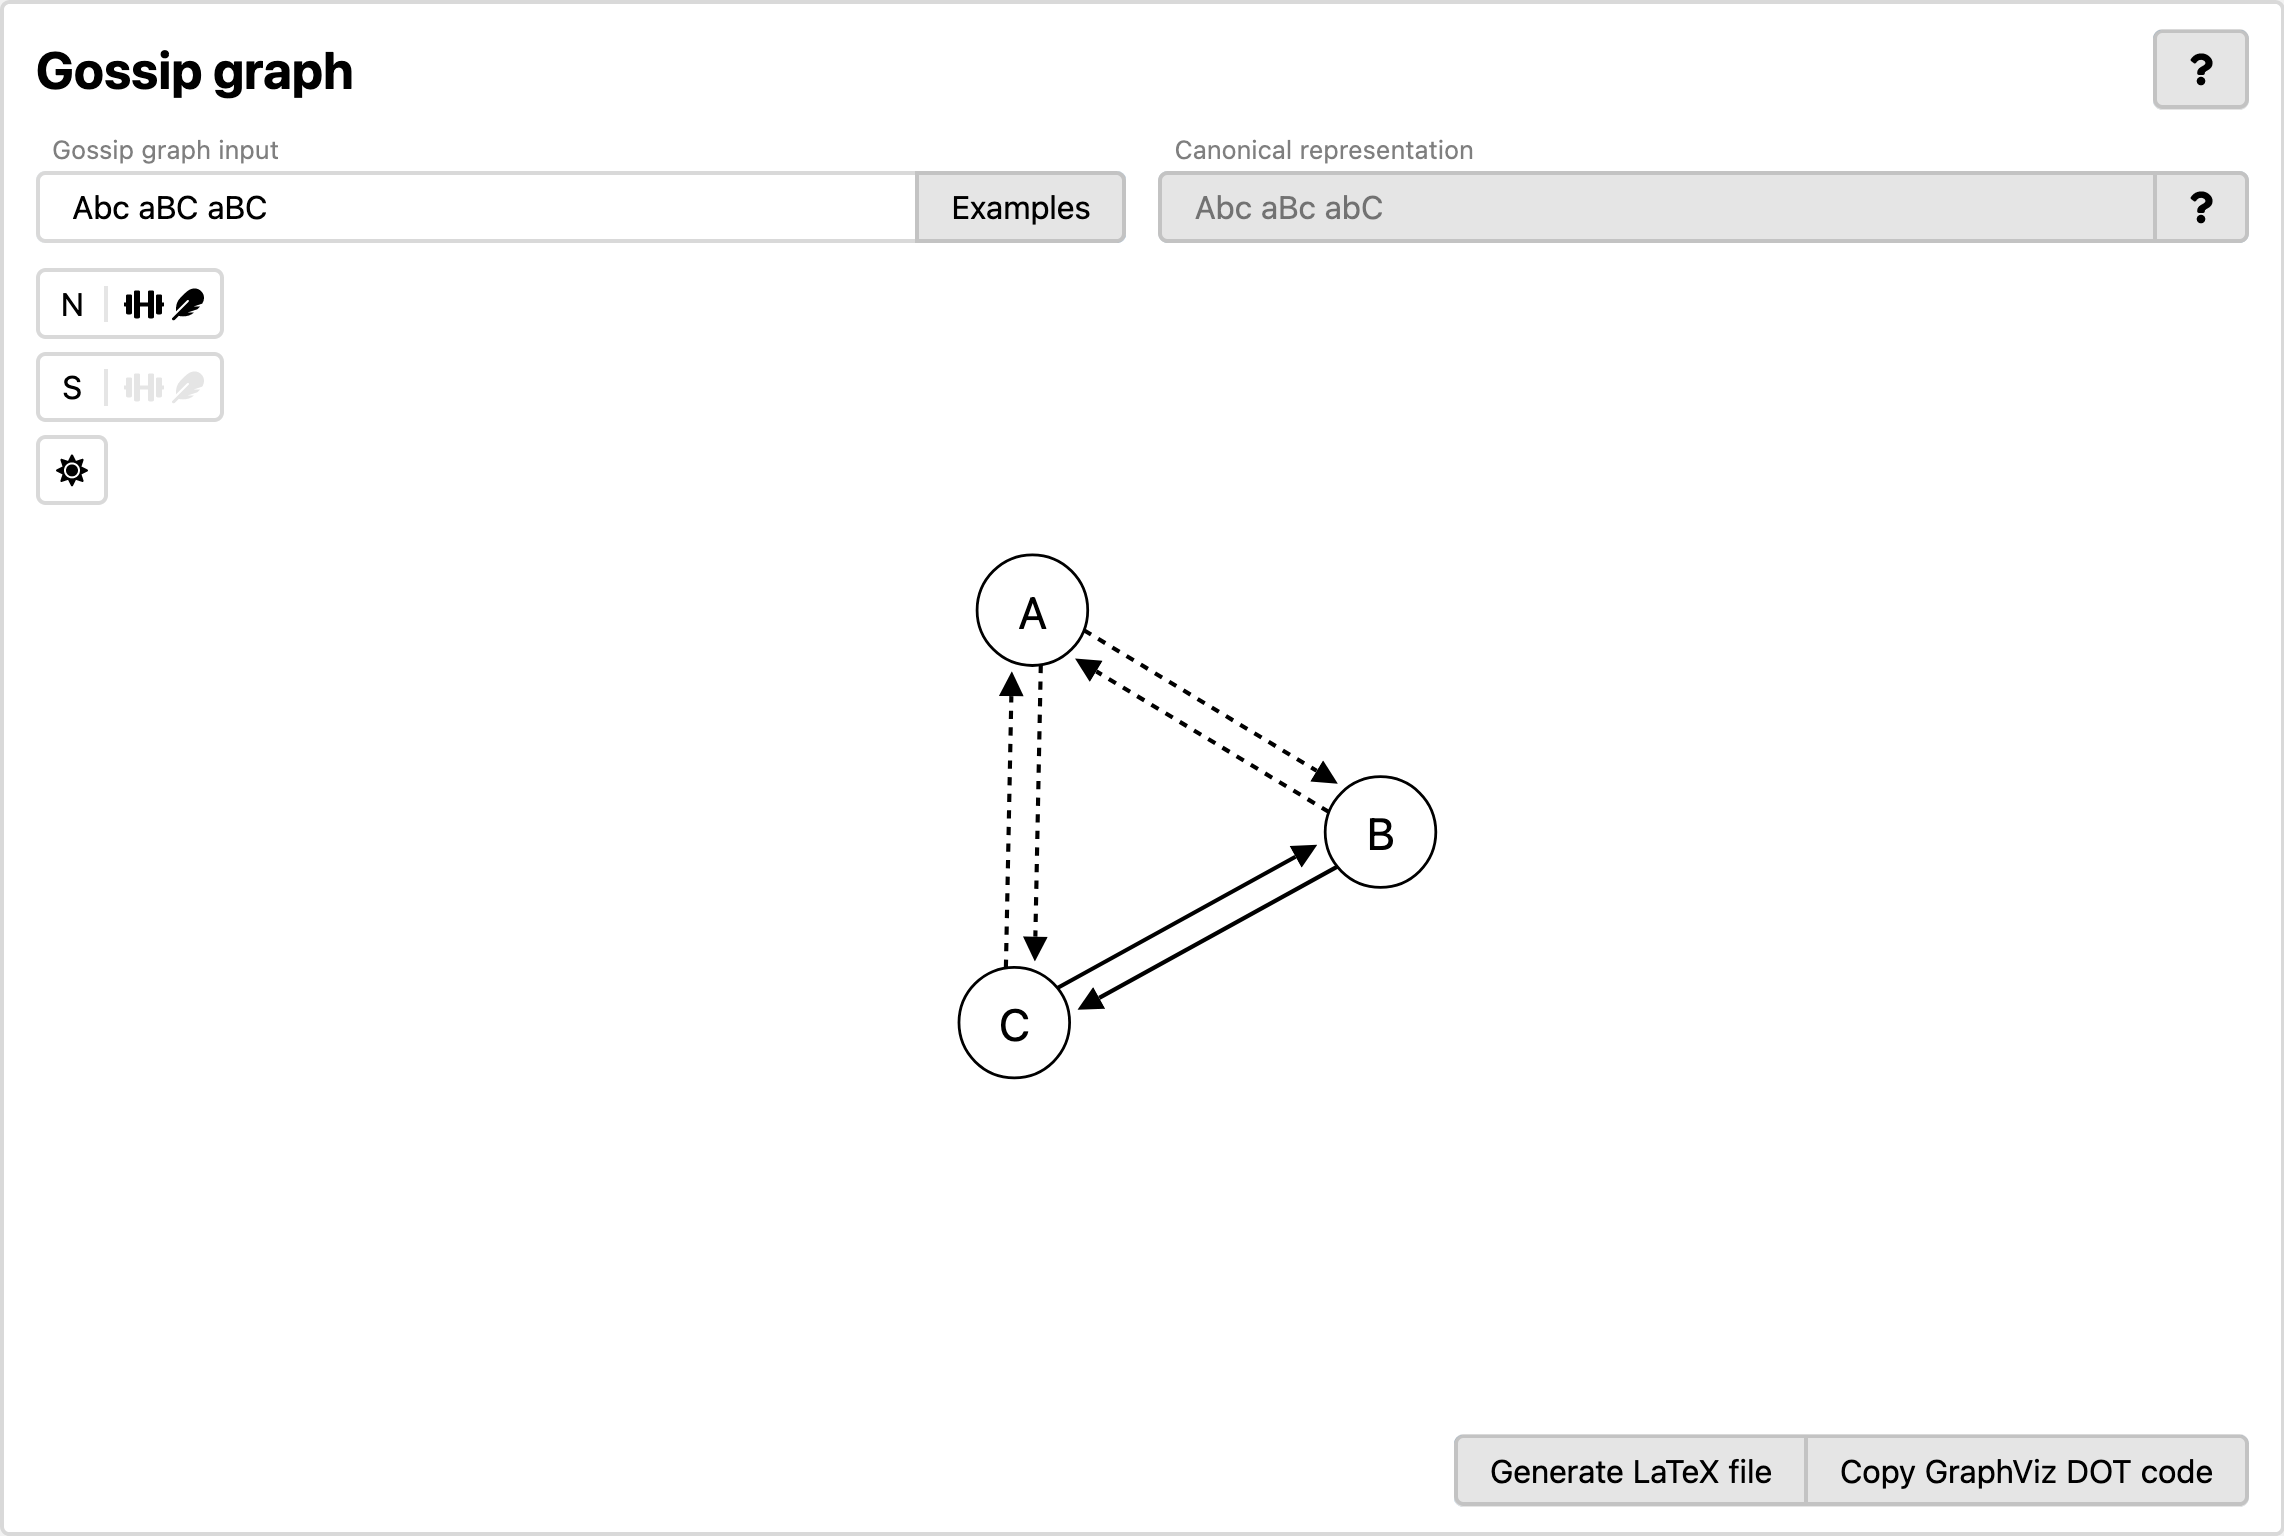
\includegraphics[width=\linewidth]{img/gossip-graph.png}
    \caption{A visualised gossip graph. Users enter the text representation of the gossip graph on the left. The icons below this input field represent whether the number relation (N) and secret relation (S) are weakly (feather icon, Definition~\ref{def:weakly-connected}) and/or  strongly (dumbbell icon, Definition~\ref{def:strongly-connected}) connected. The sun icon represents whether the graph is a sun graph (Definition~\ref{def:sun-graph}).}
    \label{fig:gossip-graph}
\end{figure*}

One of the easiest ways to visualise connections in a network is by using a graph.
Therefore, the application is able to visualise gossip graphs based on user input.
The input is provided by users in text, and uses a format based on the one used in the appendix of \textcite{van_ditmarsch_strengthening_2019}.
Since no complete grammar of that format is given,
the format has been adapted to be a bit more permitting than could be expected based purely on its description.
For example, our implementation considers the inputs \texttt{Abc aBc abC} and \texttt{Abc Bac Cab} the same, while the original format (arguably) would only accept the first input.

The basic idea behind the format is that every agent is represented by a letter segment.
The letters in this segment represent the relations of the agent represented by that segment.
Uppercase letters represent the secret relation \(S\) and lowercase letters represent the number relation \(N\).
Because every agent knows their own secret (\(I_A \subseteq S\)), it is possible to find names for all agents if and only if the input represents a valid gossip graph.
That is, every agent is represented by some letter segment such that the number of segments is equal to the number of unique agent names, and every letter segment contains a secret relation that allows it to be uniquely identified.
This procedure is described in more detail in Algorithm~\ref{alg:find-agents}.

\begin{algorithm*}
    \SetKwInOut{Input}{input}
    \SetKwInOut{Output}{output}
    \SetKwFunction{Up}{GetUppercaseLetters}
    \SetKwFunction{Error}{ShowError}
    \SetKwData{Names}{names}
    \SetKwData{Segments}{segments}
    \SetKwData{Segment}{segment}
    \SetKwData{PosNames}{possibleNames}
    \SetKwData{Name}{name}
    \SetKwData{Unique}{UniqueNameFound}
    \DontPrintSemicolon

    \Input{A list of letter sequences called \Segments}
    \Output{A list of agent names}
    \Names $\leftarrow$ \{\}\;
    \ForEach{\Segment $\in$ \Segments}{
        \PosNames $\leftarrow$ \Up{\Segment}\;
        \Unique $\leftarrow$ false\;
        \ForEach{\Name $\in$ \PosNames}{
            \If{\Name $\notin$ \Names}{
                \Names $\leftarrow \{\Name\} \cup \Names$\;
                \Unique $\leftarrow$ true\;
            }
        }
        \BlankLine
        \If{$\neg $\Unique}{
            \Error{}\;
        }
    }
    \BlankLine
    \Return{\Names}\;
    \caption{Finding agent names.}\label{alg:find-agents}
\end{algorithm*}

Once the agent names have been found, it is possible to parse the relations from the input string.
Algorithm~\ref{alg:find-agents} assumes the first agent name it finds represents the first agent. 
Thus, the first segment represents the relations of that agent.

This interpretation of the format is likely a bit more permissive than the original format.
For example, in the original format, the names of agents always follow alphabetic order -- agent 1 is A, agent 2 is B, et cetera.
Furthermore, the text segments in the original format are always ordered alphabetically.
These requirements are not present in the implementation, so an input like \texttt{Xyz Yzx Zxy} is allowed.
However, the tool does generate a ``canonical string representation'' which does follow the original rules.

\subsubsection{Executing calls}
\label{sec:protocol-execution}

\paragraph{Single calls}
\label{sec:call-execution}

When a gossip graph is given by the user, the tool allows them to execute calls and call sequences. 
Because the possible calls depend on the active protocol,
a list of possible calls is given for the currently active protocol (Figure~\ref{fig:protocol-creator}).
The possible calls are found by checking for call permissibility as defined in Definition~\ref{def:call-permissibility}.
When the user clicks one of these calls, the call is executed.
The call then happens according to Definition~\ref{def:call-effect-graph}.

\paragraph{Call sequences}
\label{sec:call-sequence-executiun}

\begin{figure}[htb!]
    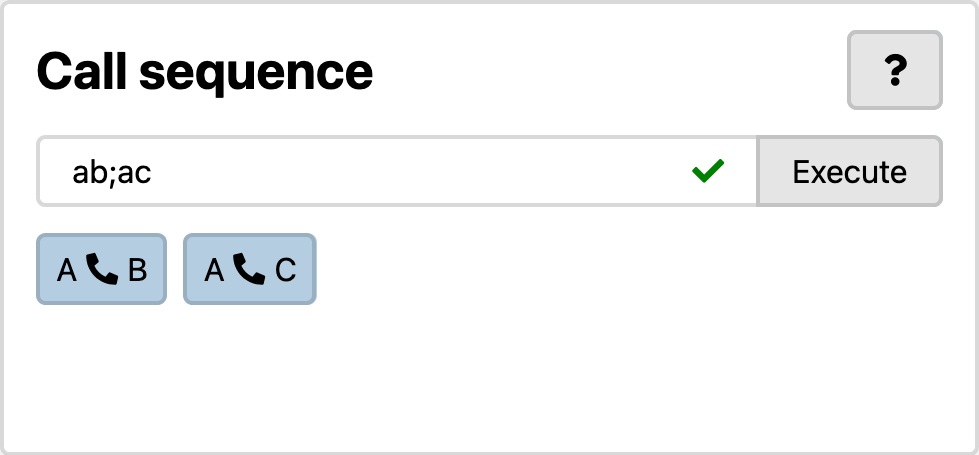
\includegraphics[width=\linewidth]{img/call-sequence.png}
    \caption{The interface for evaluating and executing call sequences. The check indicates the entered call sequence is possible and permissible.}
    \label{fig:call-sequence}
\end{figure}

It is also possible to execute entire call sequences.
The user is able to enter a call sequence using a text input according to the format given in Definition~\ref{def:call-sequence} (Figure~\ref{fig:call-sequence}).
This sequence is then checked for possibility (Definition~\ref{def:call-sequence-possibility}) and permissibility (Definition~\ref{def:call-sequence-permissibility}).
It should be noted that these checks are done in the order mentioned here.
This means that the user receives feedback on their input when they enter a call sequence that is not possible on the current gossip graph.
This has the added advantage that the system need not check for permissibility if the user enters a call sequence that is impossible.
Additionally, because possibility is a requirement for permissibility and its check is executed before the permissibility check, this check does not need to occur in the check for permissibility;
if the system reaches the permissibility check, the call sequence is guaranteed to be possible.

\paragraph{Existing protocols}
\label{sec:existing-protocols}

The tool by default includes the gossip protocols mentioned in \textcite{van_ditmarsch_dynamic_2018}.
These are \emph{Any} (\texttt{ANY}), \emph{Call Once} (\texttt{CO}), \emph{Weak Call Once} (\texttt{wCO}), \emph{Spider} (\texttt{SPI}), \emph{Token} (\texttt{TOK}) and \emph{Learn New Secrets} (\texttt{LNS}).

\paragraph{Custom protocols}
\label{sec:custom-protocols}

To allow more flexibility in using protocols, 
our tool allows the user to create their own gossip protocols.\footnote{Note: at the time of publication, this part of the tool was not finished.}
This is done through a drag-and-drop interface,
in which users can arrange boolean constituents or groups of boolean constituents.
These constituents are then interspersed with either logical conjunction (\(\land\)) or logical disjunction (\(\lor\)) (see also Figure~\ref{fig:protocol-creator}).

\begin{figure}[htb!]
    \centering
    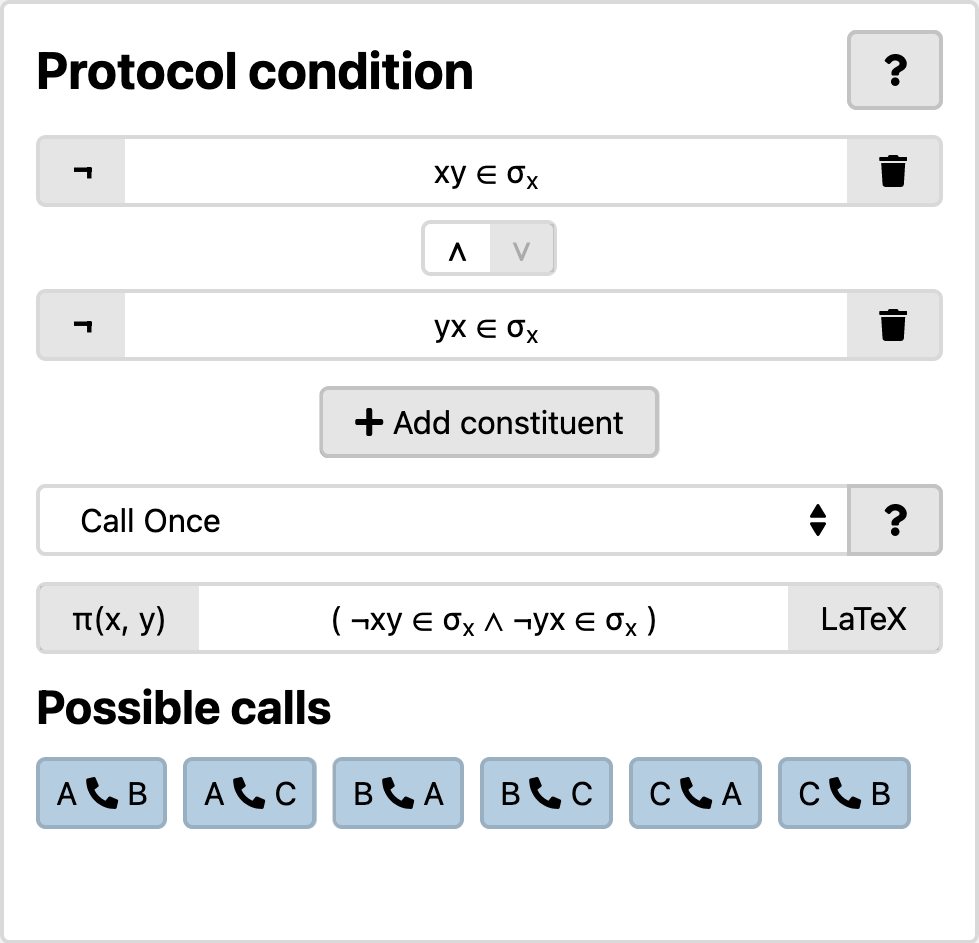
\includegraphics[width=\linewidth]{img/protocol-builder.png}
    \caption{The proposed interface for creating custom gossip protocols.}
    \label{fig:protocol-creator}
\end{figure}

The creation of custom protocols is based on the language \(\mathcal{L}_B(V)\) of boolean formulas, 
given by the Backus-Naur form:
\(\varphi ::= \top \mid p \mid \neg \varphi \mid \varphi \land \varphi\), where \(p \in V\). 
This is extended with the logical disjunction by virtue of the formula \(\varphi \lor \psi := \neg(\neg\varphi \land \neg\psi)\).
For our tool, the vocabulary \(V\) is the set of constituents of protocol conditions as defined in Definition~\ref{def:protocol-condition}.

The implementation of this functionality is based on a binary tree in which nodes can either represent constituents or connectives (\(\lor\) and \(\land\)). 
An example of this can be seen in Figure~\ref{fig:logic-tree}.
Users are able to modify the by dragging and dropping constituents to new locations,
toggling connectives between (\(\land\)) and (\(\lor\)) by clicking them,
and deleting constituents.
The application will then parse this into an Elm function which can be used to determine the possible calls.

\begin{figure}[htb!]
    \begin{subfigure}[t]{.45\linewidth}
        \centering
        \begin{tikzpicture}
            \tikzset{every tree node/.style={draw}}
            \tikzset{edge from parent/.style={draw,edge from parent path={(\tikzparentnode.south)-- +(0,-8pt)-| (\tikzchildnode)}}}
            \Tree
            [.{\( \land \)} 
                [.{\( xy \notin \sigma_x \)} ]
                [.{\( yx \notin \sigma_x \)} ]
            ]
        \end{tikzpicture}
        \caption{The \emph{Call me Once} protocol as visible in Figure~\ref{fig:protocol-creator}.}
    \end{subfigure}
    \hfill
    \begin{subfigure}[t]{.5\linewidth}
        \centering
        \begin{tikzpicture}
            \tikzset{every tree node/.style={draw}}
            \tikzset{edge from parent/.style={draw,edge from parent path={(\tikzparentnode.south)-- +(0,-8pt)-| (\tikzchildnode)}}}
            \Tree
            [.{\( \land \)} 
                [.{\( xy \in \sigma_x \)} ]
                [.{\( \lor \)} 
                    [.{\( S^\sigma xy \)} ]
                    [.{\( \sigma_x = \epsilon \)} ]
                ]
            ]
        \end{tikzpicture}
        \caption{A custom protocol (\( xy \in \sigma_x \land ( S^\sigma xy \lor \sigma_x = \epsilon ) \)).}
    \end{subfigure}
    \caption{The binary tree representation of protocol conditions.}
    \label{fig:logic-tree}
\end{figure}

\subsubsection{Execution tree}

Whenever a call or call sequence is executed, the calls are recorded on a timeline.
This timeline is displayed as the initial graph and the sequence of calls performed on it.
Users are able to navigate between different states of the gossip graph by clicking a call,
which changes the state of the gossip graph to the state it had after the clicked call.

\begin{figure}[htb!]
    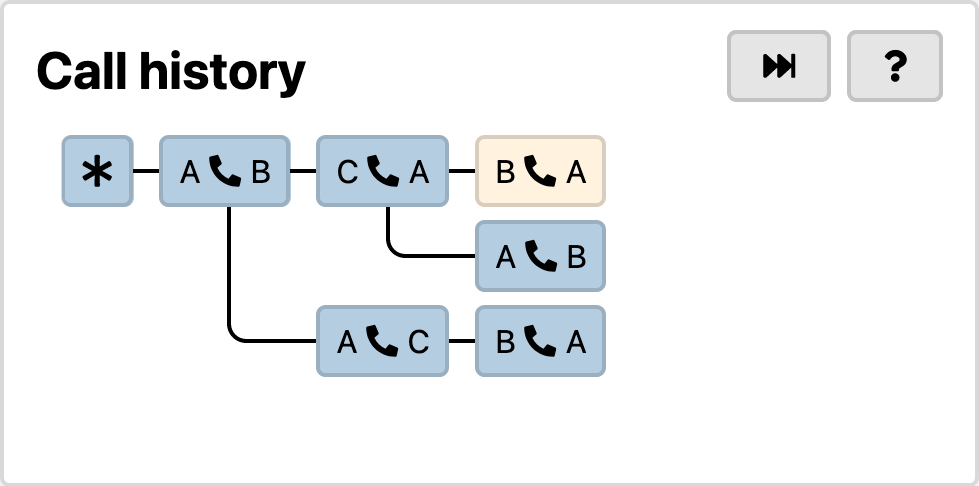
\includegraphics[width=\linewidth]{img/execution-tree.png}
    \caption{The way the execution tree is visualised in our tool. The \(*\) node represents the initial gossip graph. The yellow node represents the current `location' in the execution tree.}
    \label{fig:execution-tree}
\end{figure}

There are two ways in which the execution tree can be generated.
The first is by executing calls or call sequences.
This appends the call (or call sequence) to the current state of the gossip graph.
This allows for branching in the execution tree:
if calls have already been executed after the current state, a new branch will be added.
The second is by using the `forward' button (visible in Figure~\ref{fig:execution-tree}, the leftmost button in the top right corner).
Pressing this button will present the user with a dialog in which they can determine the maximal branching depth of the execution tree, allowing a depth of at most 5 levels.
This maximum has been implemented in order to make sure the program can calculate the execution tree, as the number of nodes to be calculated grows exponentially.
Circumstantial evidence suggests the tool can handle a depth of 5 under the \texttt{ANY} protocol given an initial graph \(G = (A = \{a, b, c\}, N = A^2, S = I_A)\) (resulting in \(6^5 = 7,776\) nodes) without much difficulty.

\subsubsection{User interaction and support}

\paragraph{Error messages}

In order to make the tool more user-friendly, it provides error messages explaining the problem when an error occurs.
An example of this can be seen in Figure~\ref{fig:errors}.

\begin{figure}[htb!]
    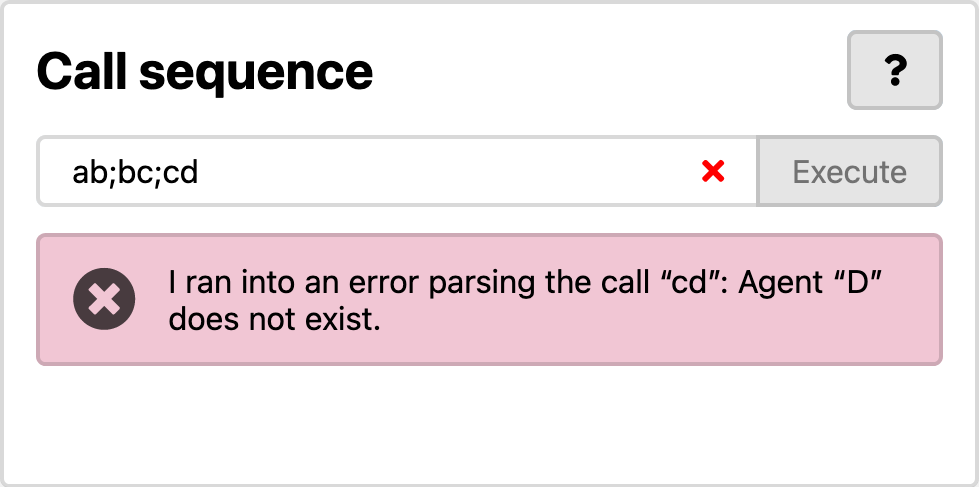
\includegraphics[width=\linewidth]{img/errors.png}
    \caption{An error that is shown when a call sequence containing a non-existing agent is entered.}
    \label{fig:errors}
\end{figure}

\paragraph{Documentation}

To make the documentation as accessible as possible, the user documentation was integrated in the user interface.
When users click the \texttt{[?]} button that is present on every section, they are shown a popup window containing an explanation of that section's functionality.
An example of this can be seen in Figure~\ref{fig:documentation}

\begin{figure}[htb!]
    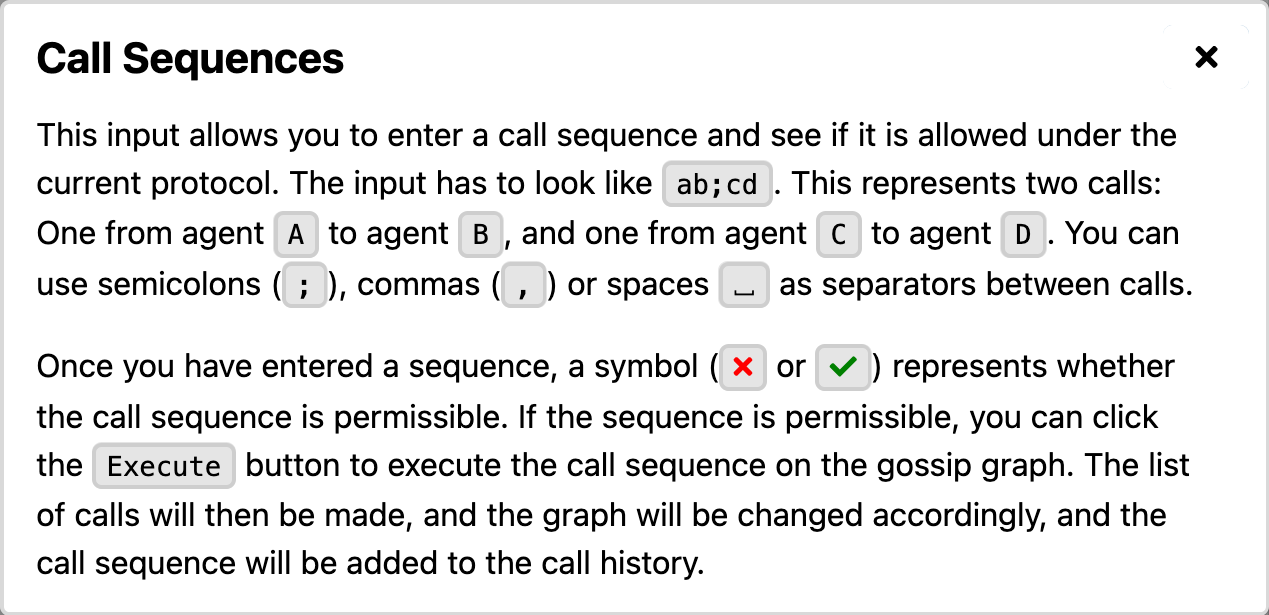
\includegraphics[width=\linewidth]{img/documentation.png}
    \caption{The documentation message for call sequences.}
    \label{fig:documentation}
\end{figure}

\subsection{Evaluation}

To evaluate the usability and applicability of the tool,
a short exploratory survey was sent out to a number of researchers active in the field of (dynamic) gossip as well as students of the master course ``Design of Multi-Agent Systems'' at the University of Groningen.
The purpose of this survey was to evaluate the ease of use and applicability of the tool,
to identify most important features and to gather suggestions for improvement and/or extensions.
The questions used can be found in Appendix~\ref{ap:survey}.

The response types for this survey are semantic differential scales, Yes/No/Maybe questions, multiple-choice lists and open-input questions. The semantic differential scales will be analysed using a Wilcoxon Rank Sum test (sometimes also known as a Mann-Whitney U-test). 
The responses will be treated as an interval scale centered around the neutral response, which is at 3.
For the Yes/No/Maybe questions, a cross table will be used.
Lastly, the open-answer questions will be paraphrased in the analysis; 
they are intended to gather possible improvements and do not contribute to the statistical analysis of the tool.